\documentclass[12pt]{beamer}
\usepackage[utf8]{inputenc}
\usetheme{default}
\usepackage{pgf,pgfarrows,pgfnodes}
\usepackage{graphicx}
\usepackage{algorithmicx} 
\usepackage{color}
\usepackage{lipsum}  
\usepackage{xcolor}
\usepackage{pdfpages}
\usepackage{hyperref}
\usepackage[english]{babel}
\usepackage{graphicx}
\usepackage{ragged2e}
\usepackage{tikz}
\usepackage{media9}
\usepackage{multirow}
\usepackage{tabularx}
\usepackage{array}
\usepackage{mathptmx}       % selects Times Roman as basic font
\usepackage{helvet}         % selects Helvetica as sans-serif font
\usepackage{courier}        % selects Courier as typewriter font
\usepackage{type1cm}        % activate if the above 3 fonts are
\usepackage{textpos} 
\usepackage{pgf,pgfarrows,pgfnodes}
\usepackage{graphicx}
\usepackage{color}
\usepackage{natbib}
\setbeamersize{text margin left=10pt,text margin right=10pt}
\definecolor{idrbt_dark_blue}{HTML}{3333b3}
\definecolor{idrbt_blue}{HTML}{00AEEF} 
\definecolor{adroit_black}{HTML}{222222}
\let\oldcite=\cite                                                              
\renewcommand{\cite}[1]{\textcolor[rgb]{0,.7,0}{\oldcite{#1}}}
\setbeamercolor{item}{fg=idrbt_blue}
\setbeamertemplate{section in toc}
{\leavevmode\leftskip=2ex%
	\llap{%
		\usebeamerfont*{section number projected}%
		\usebeamercolor{section number projected}%
		\begin{pgfpicture}{-1ex}{0ex}{1ex}{2ex}
			\color{idrbt_blue}
			%      \color{red}
			\pgfpathcircle{\pgfpoint{0pt}{.75ex}}{1.7ex}
			\pgfusepath{fill}
			\pgftext[base]{\color{fg}\inserttocsectionnumber}
		\end{pgfpicture}\kern1.25ex%
	}%
	\inserttocsection\par}
\date{}
\title{\textcolor{idrbt_blue}{\rule{112mm}{1.25mm}} \textbf{Lecture-5:\\ Operations in R, File Handling \& Visualization}
	 \textcolor{idrbt_blue}{\rule{112mm}{1.25mm}}}
\author{\textcolor{red}{\texttt{\textbf{Manu.V.T.}\\ 
			{\scriptsize Senior Research Fellow\\ Center of Excellence in Cyber Security\\IDRBT}}} }%\newline {\scriptsize Research Fellow} }
%%%%%%%%%%%%%%%%%%%%%%%%%%%%%%%%%%%%%%%%%%%%%%%%%%%%%%%%%%%%%%
\makeatletter
\long\def\beamer@section[#1]#2{%
	\beamer@savemode%
	\mode<all>%
	\ifbeamer@inlecture
	\refstepcounter{section}%
	\beamer@ifempty{#2}%
	{\long\def\secname{#1}\long\def\lastsection{#1}}%
	{\global\advance\beamer@tocsectionnumber by 1\relax%
		\long\def\secname{#2}%
		\long\def\lastsection{#1}%
		\addtocontents{toc}{\protect\beamer@sectionintoc{\the\c@section}{#2\hfill\the\c@page}{\the\c@page}{\the\c@part}%
			{\the\beamer@tocsectionnumber}}}%
	{\let\\=\relax\xdef\sectionlink{{Navigation\the\c@page}{\noexpand\secname}}}%
	\beamer@tempcount=\c@page\advance\beamer@tempcount by -1%
	\beamer@ifempty{#1}{}{%
		\addtocontents{nav}{\protect\headcommand{\protect\sectionentry{\the\c@section}{#1}{\the\c@page}{\secname}{\the\c@part}}}%
		\addtocontents{nav}{\protect\headcommand{\protect\beamer@sectionpages{\the\beamer@sectionstartpage}{\the\beamer@tempcount}}}%
		\addtocontents{nav}{\protect\headcommand{\protect\beamer@subsectionpages{\the\beamer@subsectionstartpage}{\the\beamer@tempcount}}}%
	}%
	\beamer@sectionstartpage=\c@page%
	\beamer@subsectionstartpage=\c@page%
	\def\insertsection{\expandafter\hyperlink\sectionlink}%
	\def\insertsubsection{}%
	\def\insertsubsubsection{}%
	\def\insertsectionhead{\hyperlink{Navigation\the\c@page}{#1}}%
	\def\insertsubsectionhead{}%
	\def\insertsubsubsectionhead{}%
	\def\lastsubsection{}%
	\Hy@writebookmark{\the\c@section}{\secname}{Outline\the\c@part.\the\c@section}{2}{toc}%
	\hyper@anchorstart{Outline\the\c@part.\the\c@section}\hyper@anchorend%
	\beamer@ifempty{#2}{\beamer@atbeginsections}{\beamer@atbeginsection}%
	\fi%
	\beamer@resumemode}%

\def\beamer@subsection[#1]#2{%
	\beamer@savemode%
	\mode<all>%
	\ifbeamer@inlecture%
	\refstepcounter{subsection}%
	\beamer@ifempty{#2}{\long\def\subsecname{#1}\long\def\lastsubsection{#1}}
	{%
		\long\def\subsecname{#2}%
		\long\def\lastsubsection{#1}%
		\addtocontents{toc}{\protect\beamer@subsectionintoc{\the\c@section}{\the\c@subsection}{#2\hfill\the\c@page}{\the\c@page}{\the\c@part}{\the\beamer@tocsectionnumber}}%
	}%
	\beamer@tempcount=\c@page\advance\beamer@tempcount by -1%
	\addtocontents{nav}{%
		\protect\headcommand{\protect\beamer@subsectionentry{\the\c@part}{\the\c@section}{\the\c@subsection}{\the\c@page}{\lastsubsection}}%
		\protect\headcommand{\protect\beamer@subsectionpages{\the\beamer@subsectionstartpage}{\the\beamer@tempcount}}%
	}%
	\beamer@subsectionstartpage=\c@page%
	\edef\subsectionlink{{Navigation\the\c@page}{\noexpand\subsecname}}%
	\def\insertsubsection{\expandafter\hyperlink\subsectionlink}%
	\def\insertsubsubsection{}%
	\def\insertsubsectionhead{\hyperlink{Navigation\the\c@page}{#1}}%
	\def\insertsubsubsectionhead{}%
	\Hy@writebookmark{\the\c@subsection}{#2}{Outline\the\c@part.\the\c@section.\the\c@subsection.\the\c@page}{3}{toc}%
	\hyper@anchorstart{Outline\the\c@part.\the\c@section.\the\c@subsection.\the\c@page}\hyper@anchorend%
	\beamer@ifempty{#2}{\beamer@atbeginsubsections}{\beamer@atbeginsubsection}%
	\fi%
	\beamer@resumemode}

\makeatother
%%%%%%%%%%%%%%%%%%%%%%%%%%%%%%%%%%%%%%%%%%%%%%%%%%%%%%%%%%%%%%
\beamertemplatenavigationsymbolsempty

\addtobeamertemplate{navigation symbols}{}{%
	\usebeamerfont{footline}%
	\usebeamercolor[fg]{footline}%
	\hspace{1em}%
	\insertframenumber/\inserttotalframenumber
}
%%%%%%%%%%%%%%%%%%%%%%%%%%%%%%%%%%%%%%%%%%%%%%%%%%%%%%%%%%%%%%
\begin{document}
	%%%%%%%%%%%%%%%%%%%%%%%%%%%%%%%%%%%%%%%%%%%%%%%%%%%%%%%%%%%%%%%%%%%%%%%%%%%%%%%%%%%%%%%%%%%%%%%%%%%%%%%%%%%%%%%%%%%%%%%%%%%%%
	
	\begin{frame}
	\titlepage
	


%\begin{center}
%			\begin{tabular}{l>{\centering}p{6.25cm}<{\centering}l}
%			\multirow{1}{*}{
\includegraphics[scale=0.1]{./IDRBT_lowres.png}}
%			&
%         
%			&
%			\multirow{1}{*}{
\includegraphics[scale=0.15]{./uoh.png}}
%		\end{tabular}
%\end{center}
%
\smallskip
	\renewcommand*{\arraystretch}{1.05}



\end{frame}
%%%%%%%%%%%%%%%%%%%%%%%%%%%%%%%%%%%%%%%%%%%%%%%%%%%%%%%%%%%%%%%%%%%%%%%%%%%%%%%%%%%%%%%%%%%%%%%%%%%%%%%%%%%%%%%%%%%%%%%%%%%%%

\begin{frame}
\frametitle{Outline}
\tableofcontents %[hideallsubsections]
\end{frame}
%%%%%%%%%%%%%%%%%%%%%%%%%%%%%%%%%%%%%%%%%%%%%%%%%%%%%%%%%%%%%%%%%%%%%%%%%%%%%%%%%%%%%%%%%%%%%%%%%%%%%%%%%%%%%%%%%%%%%%%%%%%%%

%%%%%%%%%%%%%%%%%%%%%%%%%%%%%%%%%%%%%%%%%%%%%%%%%%%%%%%%%%%%%%%%%%%%%%%%%%%%%%%%%%%%%%%%%%%%%%%%%%%%%%%%%%%%%%%%%%%%%%%%%%%%%
\begin{frame}
\section{Revisiting R Datatypes}
\frametitle{Revisiting R Datatypes }
			\includemedia[activate=pageopen,width=1\textwidth,height=0.75\textheight,addresource=DataTypes.mp4,flashvars={source=DataTypes.mp4 &autoPlay=true &loop=true &scaleMode=letterbox}]{}{VPlayer.swf}
	
\end{frame}
%%%%%%%%%%%%%%%%%%%%%%%%%%%%%%%%%%%%%%%%%%%%%%%%%%%%%%%%%%%%%%%%%%%%%%%%%%%%%%%%%%%%%%%%%%%%%%%%%%%%%%%%%%%%%%%%%%%%%%%%%%%%%

\begin{frame}[fragile]
\frametitle{Variable Information in R}
\section{Variable Information in R}
\begin{itemize}\justifying
	\item is.na (x) \hfill\# To identify missing values
	\item is.array(x) \hfill\# To store one, two or more dimension data
	\item is.vector(x) \hfill\# One dimension array
	\item is.matrix \hfill\# Two dimension array
	\item is.data.frame(x)
	\item is.numeric(x)
	\item is.complex(x)
	\item is.character(x)
	\item length(x)  \hfill\# Length of vector
	\item dim(x)  \hfill\# Dimension of matrix
	\item dimnames(x)  \hfill\# Dimension names
\end{itemize}
\end{frame}

%%%%%%%%%%%%%%%%%%%%%%%%%%%%%%%%%%%%%%%%%%%%%%%%%%%%%%%%%%%%%%%%%%%%%%%%%%%%%%%%%%%%%%%%%%%%%%%%%%%%%%%%%%%%%%%%%%%%%%%%%%%%%

\begin{frame}
\frametitle{Variable Conversion}
\begin{itemize}
	\item as.vector(x)
	\item as.matrix(x)
	\item as.data.frame(x)
	\item as.character(x)
\end{itemize}
\end{frame}

\begin{frame}[fragile]
\frametitle{Missing Values}
\section{Missing Values}
\begin{itemize}\justifying
	\item Variables of each data type (numeric, character, logical) can also take the
	value \textcolor{red}{NA}: not available.
	\begin{itemize}
		\item NA is not the same as 0
		\item NA is not the same as ``''
		\item NA is not the same as FALSE
	\end{itemize}
\item For any operations (calculations, comparisons) that involve NA, we have to
logically indicate whether missing values should be considered or removed.
\end{itemize}
\begin{verbatim}
> NA==1
[1] NA
> 1+NA
[1] NA
> max(c(NA, 4, 7))
[1] NA
> max(c(NA, 4, 7), na.rm=T)
[1] 7
\end{verbatim}
\end{frame}

\begin{frame}[fragile]
\section{Data selection and manipulation}
\frametitle{Data selection and manipulation }
\begin{itemize}\justifying
	\item \textbf{Slicing and Extracting Data : Vectors}
	\begin{itemize}\justifying
		\item \verb|x[n]| \hfill \# nth element
		\item  \verb|x[-n]| \hfill \# all but nth element
		\item  \verb|x[1:n]| \hfill \# first n element
		\item  \verb|x[-c(1:n)]| \hfill \# elements from n+1 to end
		\item  \verb|x[c(2,5,7)]| \hfill \# specific elements
		\item  \verb|x[x>5]| \hfill \# all elements greater than 5
		\item  \verb|x[x<9]| \hfill \# all elements less than 9
		\item  \verb|x[x>5 & x < 9]| \hfill \# all elements between 5 and 9
		\item  \verb|x[x %in% c("ab","sh")]| \hfill \# elements in given vector
	\end{itemize}
\end{itemize}
\end{frame}

\begin{frame}[fragile]
\frametitle{Data selection and manipulation }
\begin{itemize}\justifying
	\item \textbf{Data selection from list and data frame}
	\begin{itemize}\justifying
		\item \verb|x[[n]]| \hfill \# nth element of the list
		\item  \verb|x$name| \hfill \#  extract x attribute with variable name
		\item  \verb|attributes(x)| \hfill \# attributes of data frame
	\end{itemize}
\end{itemize}
\end{frame}

\begin{frame}[fragile]
\frametitle{Basic Matrix operation }
\begin{itemize}\justifying
	\item \textbf{Matrix curation }
	\begin{itemize}\justifying
		\item \verb|x[r,c]| \hfill \# element at rth row and cth column
		\item  \verb|x[r,]| \hfill \#  row r
		\item  \verb|X[,c]| \hfill \# column c
		\item  \verb|x[c(2,5,8)]| \hfill \# To select specific column	
	\end{itemize}
\end{itemize}
\end{frame}

\begin{frame}[fragile]
\frametitle{Basic Matrix operation }
\begin{itemize}\justifying
	\item \textbf{Matrix operation }
	\begin{itemize}\justifying
		\item \verb|dim(x) | \hfill \# Dimesnion of matrix
		\item \verb| x+y| \hfill \# Sum of matrix x and y
		\item \verb| dim(x) | \hfill \# Dimesnion of matrix
		\item \verb| t(x) | \hfill \# Transpose of matrix
		\item \verb| diag(x) | \hfill \# Diagonal element of matix
		\item \verb| nrow(x) | \hfill \# numer of rows
		\item \verb| rownames(x) | \hfill \# row names
		\item \verb| rowSums(x) | \hfill \# row sum
		\item \verb| rowMeans(x) | \hfill \# row means
		\item \verb| cor(x) | \hfill \# correlation matirx
		\item \verb| var(x) | \hfill \# variance matirx		
	\end{itemize}
\end{itemize}
\end{frame}

\begin{frame}[shrink=10,fragile]
\frametitle{Data selection and manipulation}
\begin{itemize}\justifying
	\item \textbf{Matrix operation }
	\begin{itemize}\justifying
		\item \verb| X*2 | \hfill \# scalar multiplication
		\item \verb| length(x) | \hfill \# length of the vector
		\item \verb| sum (x) | \hfill \# sum of element in vector
		\item \verb| max, min | \hfill \# max and min values
		\item \verb| rev | \hfill \# reverse in order
		\item \verb| sort | \hfill \# sorting
		\item \verb| unique | \hfill \# unique
		\item \verb| rle | \hfill \# run length encoding
		\item \verb| table(a,b) | \hfill \# comparison table
		\item \verb| sample(x) | \hfill \# for random sampling of the data
		\item \verb| which.max(x) | \hfill \# return index of the max elements of x.
		\item \verb| Which.min(x) | \hfill \# return index of the min elements of x.
		\item \verb| Which (x == a) | \hfill \# returns a vector of indices of x, if
		comparsion operator is TRUE
		\item \verb| Which (x %in% a) | \hfill \# return index which matches with a
		\item \verb| choose (n,k) | \hfill \# combinations of k events among n repetitions.
		\item \verb| rank(x) | \hfill \# ranking
		\item \verb| round(x,3) | \hfill \# round the element of x to 3 decimal places
	\end{itemize}
\end{itemize}
\end{frame}

\begin{frame}
\begin{center}
	\begin{block}{}
		\hspace*{2in}\textbf{\LARGE \textcolor{idrbt_blue}{Hands On}}
\end{block}\end{center}
\end{frame}

\begin{frame}[fragile]
\section{Hands On}
\begin{itemize}\justifying
	\item \textbf{Exercise 1}: Round off the number 3.543321 up to three
	decimal place.
	\item  \textbf{Exercise 2}: Generate a sequence, x=seq(1,524,d). where
	d is a random number between 2 to 9. Find
	\begin{itemize}\justifying
		\item length(x)
	\item sum(x)
	\item cube root of x
	\item extract 5, 7th element from vector x
	\item extract 2nd to 5th element from vector x
	\item create vector without 2nd to 5th element from
	vector x
	\item which elements of vector x are greater than 10
	\item find a vector whose elements are greater than 10
	\item find a vector whose elements are greater than 10
	and less than 50
	\item find: max, min, rev, sort, unique, range	
	\end{itemize}	

\end{itemize}
\end{frame}


\begin{frame}[fragile]
\begin{itemize}\justifying
	\item  \textbf{Exercise 3}: Explore the commands
	\begin{itemize}\justifying
		\item a=rep(2,5)
		\item b=rep(3,7)
		\item c=rep(4,2)
		\item z2= c(a,b,c)
		\item z= sample(z2) \# analyze z
		\item u = rle(z)
		\item sort (z)
		\item unique (z)
		\item what sample command does?
		\item attributes of u
		\item analyze u \# Interpret what rle does
		\item mean, median, var,sd,
		\item convert z into log scale
	\end{itemize}	
	
\end{itemize}
\end{frame}


\begin{frame}[fragile]
\begin{itemize}\justifying
	\item \textbf{Exercise 4}: Generate 20 replicate of TRUE sample
	denoted by T, and 10 replicate of FALSE sample denoted
	by F.
	\item \textbf{Exercise 5}: Generate a vector z1 from 2 to 5, second
	vector z3 from 12 to 15, and combine them into a new
	vector z.
	\item \textbf{Exercise 6}: Write the sequence expression for
	– 5 10 15 20 25 30 35 40 45 50
	\item \textbf{Exercise 7}: Generate a sequence start with 19 to 957,
	with a difference of 17.
	\item \textbf{Exercise 8}: Generate any 3$\times$4 matrix using command
	matrix
	\item \textbf{Exercise 9}: Ceate 3 vectors, a,b,c of size 5, generate a
	matrix using cbind and rbind, calculate the dimension of
	matrix.
\end{itemize}
\end{frame}

\begin{frame}[fragile]
\begin{itemize}\justifying
	\item \textbf{Exercise 10}: A class of 20 student, appeared for maths
	and biology exam, secure marks between 20 to 90.
	Genearte random marks, satisfying the above criteria in a
	matrix, that contain First Row as name of the student as
	S1, S2, ...., S20, and first column as the subject math1
	and bio1 respectively.
	Save the name of the students and marks of the student
	who,
	\begin{itemize}\justifying
	\item Secure more than 70 \% marks in either of two
	subjects, and
	\item  Fail in either of two.
	\item  Average marks secure by students in both subjects
\end{itemize}
\end{itemize}
\end{frame}

\begin{frame}
\begin{center}
	\begin{block}{}
		\hspace*{2in}\textbf{\LARGE \textcolor{idrbt_blue}{File Handling}}
\end{block}\end{center}
\end{frame}


\begin{frame}
\frametitle{Reading text files}
\begin{itemize}\justifying
	\item Most text data files are in ASCII format and are usually
	produced by a text editor such as gedit or Notepad.
	\item  The \textcolor{red}{read.table( )} function allows us to convert data
	available in an external text directly into a data frame.
	In the following example, we use the text file
	\item  A data frame is an R object very similar in appearance
	to a matrix object except that columns in a data frame
	can be of different types: numeric or character.
\end{itemize}
\end{frame}

\begin{frame}[fragile]
\frametitle{Reading text files}
\begin{itemize}\justifying
	\item \verb|data<-read.table("C:sample.data.txt")|
	\item \verb|data<-read.table("/home/manuvt/sample.data.txt")|
	\item data$<-$read.table("http://183.82.43.252/~manu/sample\_data.txt”)
	\item Read from excel 
	\begin{itemize}
		\item Read.delim (``clipboard”)
		\item \verb|x=read.delim("clipboard",header=TRUE)|
	\end{itemize}
\end{itemize}
\end{frame}

\begin{frame}[fragile]
\frametitle{Create a sample file}
\begin{itemize}\justifying
	\item First we read a very short data file. The data file is
	called \textcolor{red}{simple.csv} and has three columns of data and six
	rows. The three columns are labeled "trial," "mass," and
	"velocity."
	\item A copy of the data file is shown below
	\begin{verbatim}
		"trial","mass","velocity"
	"A",10,12
	"A",11,14
	"B",5,8
	"B",6,10
	"A",10.5,13
	"B",7,11
	\end{verbatim}
\end{itemize}
\end{frame}

\begin{frame}
\begin{itemize}
	\item We assume that the data file is in the format called "comma
	separated values" (csv). That is, each line contains a row of values
	which can be numbers or letters, and each value is separated by a
	comma.
	\item	It is possible to save an Excel spreadsheet as a csv file.
	We also assume that the very first row contains a list of labels. 
		\item	The	idea is that the labels in the top row are used to refer to the
	different columns of values.
\end{itemize}
\end{frame}

\begin{frame}
The command to read the data file is \textcolor{red}{read.csv}.
\begin{itemize}
	\item The first argument is the name of file.
	\item The second argument indicates whether or not the first row
	is a set of labels.
	\item The third argument indicates that there is a comma between
	each number of each line.
\end{itemize}

The following command will read in the data and assign it to a
variable called sample.\\
\textcolor{red}{simple =
read.csv(file="sample.csv",head=TRUE,sep=",")}
\end{frame}

\begin{frame}
\begin{itemize}\justifying
	\item The variable simple contains the three columns of data. Each
	column is assigned a name based on the header (the first line in
	the file).
	\item You can now access each individual column using a "\$" to
	separate the two names:\\
	simple\$trial\\
	simple\$mass\\
	simple\$velocity
	\item If you are not sure what columns are contained in the variable
	you can use the \textbf{names} command:\\ \textbf{names(simple)}
\end{itemize}
\end{frame}

\begin{frame}[fragile]
\frametitle{Read from file}
\begin{verbatim}
> read.table(“file”,header=TRUE)
> read.table(“file”,header=FALSE)
> read.csv(“file”,header=TRUE, sep=”,”)
> read.delim(“file”,header=TRUE,sep=”\”)
> read.delim(“file”,header=TRUE,sep=”\”, ........)
programming File
\end{verbatim}
\end{frame}

\begin{frame}[fragile]
\frametitle{Write.table}
\begin{verbatim}
write.table(x, file = "", append = FALSE, 
quote = TRUE, sep = " ",
eol = "\n", na = "NA", dec = ".", 
row.names = TRUE,
col.names = TRUE, 
qmethod = c("escape", "double"),
fileEncoding = "")

> write.table(data_variable,“file_name”,
quote = TRUE, sep = “ ”, row.names = TRUE,
 col.names = TRUE)
> write.csv(data_variable,“file_name”,........)
\end{verbatim}
\end{frame}

\begin{frame}
\begin{center}
	\begin{block}{}
		\textbf{\LARGE \textcolor{idrbt_dark_blue}{Graphics and Data Visualization}}
\end{block}\end{center}
\end{frame}

\begin{frame}
	\frametitle{Graphics in R}
\begin{itemize}
	\item R has exceptionally high quality graphics
		\item Integrated graphics and statistics infrastructure
		\item Powerful environment for visualizing scientific data
		\item Fully programmable \& Highly reproducible
		\item Vast number of R packages with graphics support
		\item Publication quality graphics
		\item R allows for fully customisable plots
		\item R allows for interactive plotting
\end{itemize}
\end{frame}

\begin{frame}[fragile]\frametitle{Graphics Environment}
\begin{itemize}
	\item Viewing graphics in R (On-screen graphics) : A graph is created by using a
	plotting command (plot, boxplot, hist, etc.) will typically overwrite a previous graph.
	To avoid this, open a new graph window before creating a new graph.
	\item Saving the graphs:	Postscript, pdf, svg, png, tiff, jpeg
	

\begin{verbatim}
> postscript(“file_name.ps”, width = 4.0, 
			height = 3.0, horizontal = FALSE)
> jpeg(“file_name.jpeg”,...............) 
> png(“file_name.png”,.................)
> tiff(“file_name.tiff”,..............) 
> bmp(“file_name.bmp”,...............)
> pdf(“file_name.pdf”,..................)
\end{verbatim}

\item Close : graphics device\\
\verb|> dev.off()|
\end{itemize}
\end{frame}

\begin{frame}[fragile]
\begin{verbatim}
plot(x1.new, y1.new, col="red", type="b", 
pch =21, lty=2, lwd=1, ylim=c(0,60),
xlim=c(-0.4,0.2), bg="slateblue3" 
xlab=”XLabel”,ylab=”YLabel”, main=”Main Title”)
\end{verbatim}
\end{frame}

\begin{frame}
\frametitle{Graphics Parameters}
\begin{tabular}{l|l}
	\textbf{Function} &\textbf{Description}\\ \hline
	col &Color of line , text\\
	lwd &Line width\\
	lty &Line type\\
	font &Font face (plain, bold, italic)\\
	pch &Type of plotting symbol\\
	srt &String rotation\\
\end{tabular}
\end{frame}

\begin{frame}[fragile]\frametitle{Graphics Parameters}
Graph has many features (font, color, axis, title, etc.) can be assessed through
function \textbf{par()}. Change in par function will be in effect for the rest of the session or until we
change tham again.
\begin{verbatim}
par() # view current settings
opar <- par() # make a copy of current settings
par(col.lab="red") # red x and y labels
hist(mtcars$mpg) # create a plot with these new settings
par(opar) # restore original settings
\end{verbatim}
\end{frame}

\begin{frame}
\frametitle{Text and Symbol Size}
\begin{tabular}{lp{0.75\textwidth}}
	\textbf{Option} &\textbf{Description}\\
	cex &number indicating the amount by which plotting text and
	symbols should be scaled relative to the default.
	1=default, 1.5 is 50\% larger, 0.5 is 50\% smaller, etc.\\
	cex.axis &magnification of axis annotation relative to cex\\
	cex.lab &magnification of x and y labels relative to cex\\
	cex.main &magnification of titles relative to cex\\
	cex.sub &magnification of subtitles relative to cex\\
\end{tabular}
\end{frame}

\begin{frame}
\frametitle{Plotting Symbol}
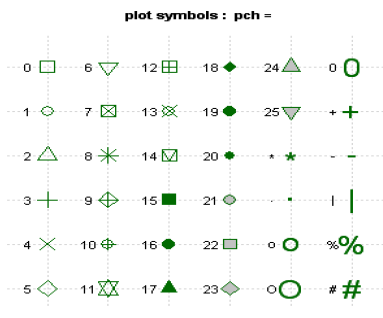
\includegraphics[scale=0.5]{pch}
\end{frame}

\begin{frame}
\frametitle{Lines}
\begin{itemize}
	\item Reference line, axes, and fit lines can be chnage by :
\end{itemize}
\begin{tabular}{lp{0.85\textwidth}}
	\textbf{Option} &\textbf{Description}\\
lty &line type. see the chart below.\\
lwd &line width relative to\\	
\end{tabular}
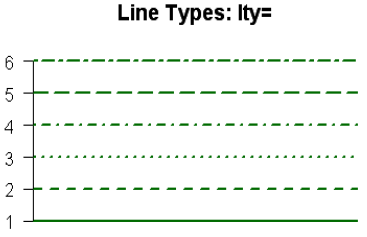
\includegraphics[scale=0.5]{line}
\end{frame}

\begin{frame}
\frametitle{Multiple Figures : Combining Plots}
R make it easy to combine multiple plots into one graphs, using either the \textbf{par()} or
\textbf{layout()} function.
\begin{itemize}
	\item  \textbf{par()}, we can include\textbf{ mfrow =c (nrows, ncols)}, to create a matrix of
	nrows and ncols plot that are filled in by row.
	\item   .................... mfcol =c (nrows, ncols) filled by column.
	\item  \textbf{layout()} function has the form \textbf{layout(mat)} where mat is the matrix
	object specifying the location of N figure to plot.
\end{itemize}
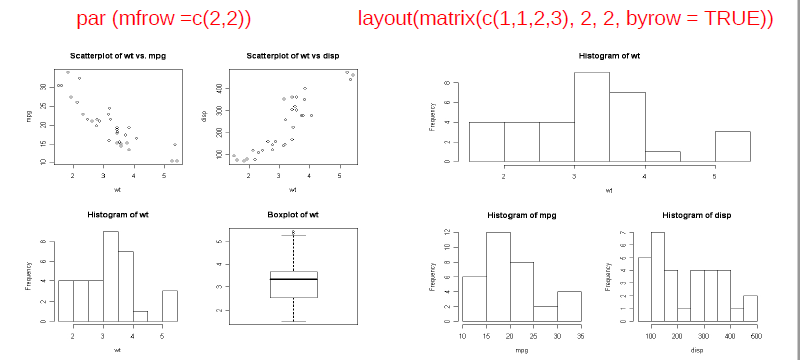
\includegraphics[scale=0.35]{multifig}
\end{frame}


\begin{frame}
\frametitle{Text Annotations}
\begin{itemize}
	\item Text can be added to graph using
	\begin{itemize}
		\item \textbf{text()}, to place text within graph
	\end{itemize}
\end{itemize}
\begin{tabular}{lp{0.85\textwidth}}
	\textbf{Option} &\textbf{Description}\\
	location &location can be an x,y coordinate. Alternatively, the text can be
	placed interactively via mouse by specifying location as locator(1).\\
	pos &position relative to location. 1=below, 2=left, 3=above, 4=right. If
	you specify pos, you can specify offset= in percent of character
	width.\\
	side &which margin to place text. 1=bottom, 2=left, 3=top, 4=right. you
	can specify line= to indicate the line in the margin starting with 0
	and moving out. you can also specify adj=0 for left/bottom
	alignment or adj=1 for top/right alignment.\\
	cex & as discussed earlier \\
	col & as discussed earlier \\
	font & as discussed earlier \\
\end{tabular}
\end{frame}

\begin{frame}[fragile]
\frametitle{Labeling Points}
\begin{itemize}
	\item \textbf{text()}, function can be used for labeling point as well as adding other
	text annotations.
	\item specify location as a set of x, y coordinates and specify text to place as
	a vector of labels.
\end{itemize}
\begin{verbatim}
attach(mtcars)
plot(wt, mpg, main="Milage vs. Car Weight",
xlab="Weight", ylab="Mileage", pch=18, col="blue")
text(wt, mpg, row.names(mtcars), cex=0.6, pos=4, 
col="red")
\end{verbatim}
\end{frame}


\begin{frame}[fragile]
\frametitle{Legend}
\begin{itemize}
	\item Other legend options includes bty for box type, bg for background color,
	cex for size, and text.col for text color.
		\item Setting horiz = TRUE sets the legend horizontally rather than vertically.
\end{itemize}
\begin{verbatim}
legend(location, title, legend, ...)
where legend is a character vector with the labels
\end{verbatim}
\end{frame}


\begin{frame}[fragile]
\frametitle{Interactive Plotting : identify function}
\begin{itemize}
	\item \textbf{identify()} : is a useful function which can be used to label selected points on a plot
\end{itemize}
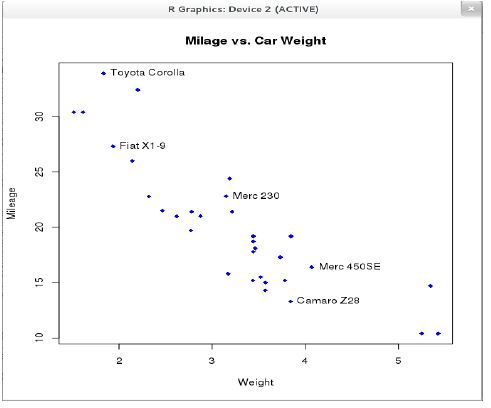
\includegraphics[scale=0.5]{identify}
\end{frame}


\begin{frame}[fragile]
\frametitle{3D - Scatter plot}
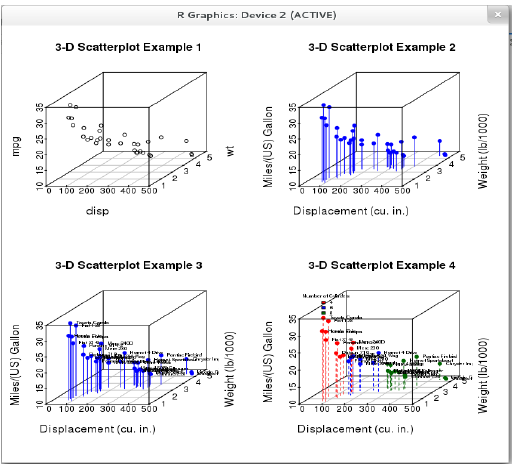
\includegraphics[scale=0.5]{3Dscatterplot}
\end{frame}

\begin{frame}[fragile]
\frametitle{Bar plot}
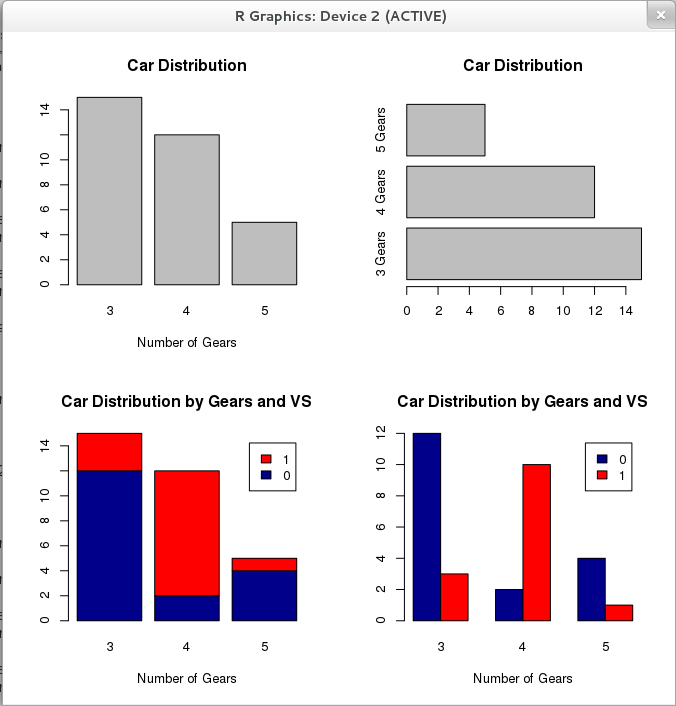
\includegraphics[scale=0.3]{barplot}
\end{frame}


\begin{frame}[fragile]
\frametitle{Histogram plot}
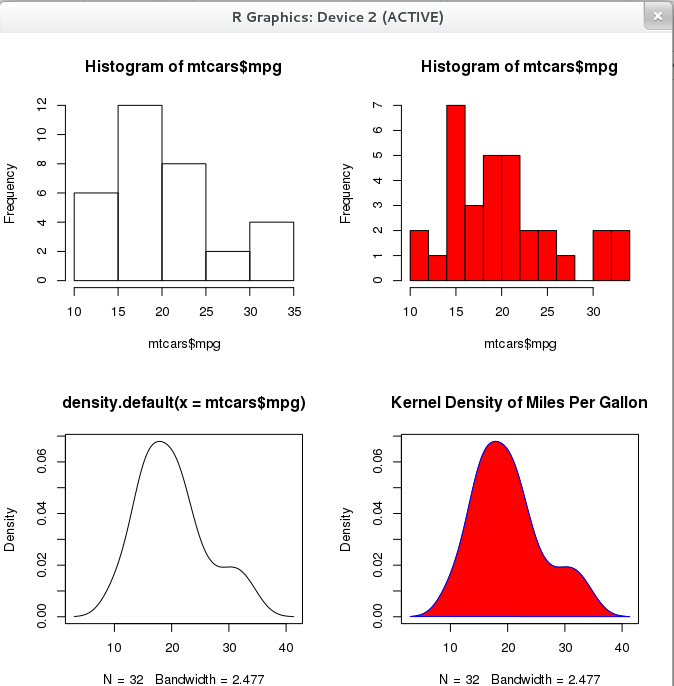
\includegraphics[scale=0.35]{histogram}
\end{frame}


\begin{frame}[fragile]
\frametitle{Pie chart}
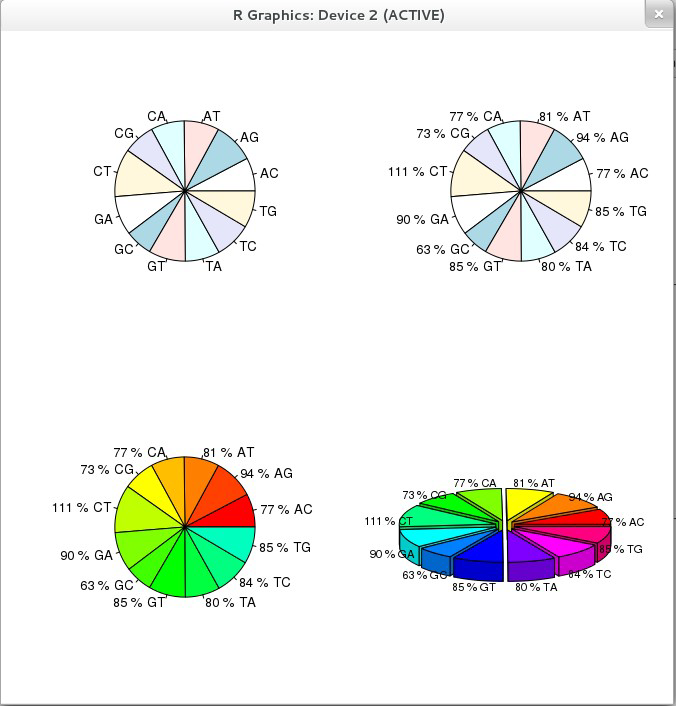
\includegraphics[scale=0.35]{piechart}
\end{frame}


\begin{frame}
 \begin{center}
\begin{block}{}
\hspace*{2in}\textbf{\LARGE \textcolor{idrbt_dark_blue}{T}\pause
			    \textcolor{idrbt_blue}{h}\pause
			    \textcolor{idrbt_dark_blue}{a}\pause
			    \textcolor{idrbt_blue}{n}\pause
			    \textcolor{idrbt_dark_blue}{k}\pause
			    \textcolor{idrbt_dark_blue}{Y}\pause
			    \textcolor{idrbt_blue}{o}\pause
			    \textcolor{idrbt_dark_blue}{u} }
\end{block}\end{center}
\end{frame}
\end{document}
%%%%%%%%%%%%%%%%%%%%%%%%%%%%%%%%%%%%%%%%%%%%%%%%%%%%%%%%%%%%%%%%%%%%%%%%%%%%%%%%%%%%%%%%%%%%%%%%%%%%%%%%%%%%%%%%%%%%%%%%%%%%%